\documentclass[11pt]{article}
\usepackage[margin=1in]{geometry}
\usepackage{amsmath,amssymb,amsthm}
\usepackage[T1]{fontenc}
\usepackage{lmodern}
\usepackage{microtype}
\usepackage{graphicx}
\usepackage{booktabs}
\usepackage[title]{appendix}
\usepackage{hyperref}
\hypersetup{colorlinks=true,linkcolor=blue,citecolor=blue,urlcolor=blue,
  pdftitle={Candidate images of Pluto on archival plates from 1908 and 1909},pdfauthor={P. Graham}}
\title{Candidate images of Pluto on archival plates from 1908 and 1909}
\author{P. Graham\\ \small\url{https://orcid.org/0009-0007-8493-1505}}
\date{November 19, 2026}
\pagestyle{plain}
\begin{document}
\maketitle
\begin{abstract}
We report candidate images of Pluto on three public plate scans from before Clyde Tombaugh discovered it in 1930: one Harvard plate exposed on December 21, 1908 (UT) and two Heidelberg plates exposed together on February 20, 1909. The Harvard plate's archived exposure midpoint is 5.8 hours later than the midpoint inferred from asteroid trails on the plate. At the inferred time each plate shows a faint, star-like image within 2 arcseconds of Pluto's predicted sky position, with a brightness consistent with Pluto's at the precision of the plates; two independent measurements agree. The earliest measurements in the Minor Planet Center's orbit fit for Pluto are from January 1914, Yerkes images of 1909 were reported without published positions, and two Harvard searches described by B.~E. Schaefer, M.~W. Buie and L.~T. Smith found no earlier image. The catalogs and comparison plates searched show no steady source bright enough to account for the images, and the nominal orbits we checked predict no known asteroid there. Shifting all three predictions by the same random offset gave no equally close match with as high a signal-to-noise ratio on all three plates in 230,352 trials. We offer the identification as a hypothesis for experts.

This work has not yet been reviewed by experts.
The proofs, the measurements, the code and the text were produced by AI models (from OpenAI and Anthropic), working under the author's direction.
\end{abstract}
\medskip
\noindent\textbf{Keywords:} Pluto, prediscovery images, archival photographic plates, DASCH, Heidelberg plate archive.

\section{Introduction}

\subsection{The finding}
Each of three public plate scans contains its own candidate image of Pluto: one Harvard plate from December 1908 and two Heidelberg plates exposed on the same night in February 1909. If the identification is correct, these images predate both the reported Yerkes images of 1909 and the accepted observations of 1914. The Harvard image appears only at the exposure time given by asteroid trails on the plate. We compare each image's position and brightness with Pluto's prediction, with comparably faint stars and with random positions on the same scans.

\begin{center}
\small
\setlength{\tabcolsep}{4pt}
\begin{tabular}{@{}lllll@{}}
\toprule
Plate & Observatory, telescope & Exposure (Universal Time) & Offset (arcsec) & Blue magnitude $B$ \\
\midrule
MA 731 & Harvard, 12-inch Metcalf & 1908 Dec 21, 00:22--01:35$^{a}$ & 0.2--0.7 & 16.0--16.2 \\
B2247a & Heidelberg, Bruce astrograph & 1909 Feb 20, 18:50--21:50 & 0.3--1.7 & 16.4--16.6 \\
B2248b & Heidelberg, Bruce astrograph & 1909 Feb 20, 18:50--21:50 & 0.9--1.9 & 16.3--16.4 \\
\bottomrule
\end{tabular}
\end{center}
\noindent\small $^{a}$ Estimated from asteroid trails on the plate; the archived midpoint is 5.8 hours later.\normalsize

\medskip
The offset is the distance of the fitted image from Pluto's predicted position at the exposure midpoint. Each range spans the values of two independent measurements (Section~\ref{sec:measure}); it is not a confidence interval. $B$ and $V$ are magnitudes in the blue and visual bands, where a larger magnitude means fainter light, and $B-V$ is their difference. Pluto's predicted $B$ on these dates is 16.3 to 16.5. Method B's values differ from it by no more than the scatter of comparably faint stars measured the same way (0.17 to 0.24 mag), and Method A's lie within its acceptance window of $\pm0.45$ mag (Section~\ref{sec:measure}).

The images lie where Pluto was predicted on each date, $0.90^\circ$ apart on the sky, so no single fixed object explains both. Catalogs show no star at either position, and other photographs sensitive enough to show a steady source of this brightness show none. In the queries and integration we ran, nominal orbits predict no known asteroid at either position; those orbits are unreliable in 1908 for many near-Earth objects, the integration covers a filtered selection, and the February check is a single query (Appendix~\ref{app:tests}). When all three predicted positions were shifted by the same random offset, none of 230,352 trials gave a match on all three plates as close as observed and with as high a signal-to-noise ratio (S/N); a looser acceptance rule is matched far more often (Section~\ref{sec:tests}). Each image is near its plate's limit, and the scans cannot exclude every alternative (Section~\ref{sec:limits}). We therefore offer the identification as a hypothesis for experts.

\subsection{Prior work}
Tombaugh found Pluto at Lowell Observatory in 1930 \cite{Tombaugh1946}. Searches of older plates followed at once, and E.~C. Bower listed 14 prediscovery images from 1914 to 1927 \cite{Bower1931,Schaefer2008}. The oldest are on two Königstuhl plates of January 23, 1914, exposed by F.~Kaiser and measured by M.~Wolf \cite{Bower1931,HDAP}. These provide the earliest measurements used in the Minor Planet Center's orbit fit for Pluto, which states ``first opposition used 1914'' \cite{MPC}. Appendix~\ref{app:history} gives other early reports.

G.~Buchwald, M.~DiMario and W.~Wild \cite{Buchwald2000,Wild1998}, of an amateur group at Yerkes Observatory, reported Pluto on the Bruce plates 6B556 and 6B583 of August 1909 and November 11, 1909. Their paper gives the August date as August 21 in its abstract and August 20 in its text. W.~Osborn and F.~Mills later re-examined both plates and considered the November image ``fairly certain'', while comparison with Palomar survey images left the August image ambiguous; a marked reproduction of the November plate was published with their account \cite{Reichhardt2015}. We found no published measured position from either plate and no full calibrated scan, and neither is in the Minor Planet Center's file \cite{MPC}. We call these images reported, and the 1914 images accepted.

Schaefer, Buie and Smith describe the Harvard searches \cite[Section~6]{Schaefer2008}. After a search in 1930, Schaefer searched again in 1982: ``A total of 65 plates (from the A, B, I, and MC series) had hopeful limiting magnitudes and covered Pluto's position at the time. Unfortunately, no prediscovery image of Pluto was identified.'' MA~731 is absent from that published list of series. In 2004 ``this search of the Harvard collection was repeated'' with ``exact positions for the minute of the middle of each plate exposure'' from JPL Horizons (the service we also use to calculate Pluto's position), made practical in part because Alison Doane ``had made a complete on-line catalog of all the deepest plates''; ``no prediscovery image was identified.'' The account lists neither the 2004 plates nor the time convention used, so we cannot say whether MA~731 was examined.

Murtagh and colleagues recently searched DASCH for prediscovery images of the trans-Neptunian object 2026~ED$_{138}$, also checking plate times against recorded sidereal times \cite{Murtagh2026}.

We add the exposure time of MA~731 from asteroid trails, at which an image appears at Pluto's position; the Heidelberg pair B2247a and B2248b, which we found in no prior report; and tests of each image against comparably faint stars, random positions on the same scans, catalogs, known asteroids and other plates.

\section{Plates, exposure times and predictions}
\label{sec:plates}

\paragraph{The plates.}
MA~731 is a plate of the Harvard MA series, taken with the 12-inch Metcalf doublet at Joel Metcalf's observatory in Taunton, Massachusetts \cite{DASCHguide}, at 97$''$ per mm. Its storage envelope records a 60-minute exposure on the local evening of December 20, 1908. DASCH \cite{Grindlay2012,Williams2025} provides the full-resolution scan, plate \texttt{ma00731}. B2247a and B2248b were taken simultaneously by A.~Kopff in the two tubes of the 16-inch Bruce astrograph on the Königstuhl, Heidelberg, both cataloged as 10,802-second exposures on blue-sensitive plates starting at 18:50:10 and 18:50:22 UT on February 20, 1909 \cite{HDAP}.

\paragraph{Exposure times from asteroid trails.}
The archived midpoint of MA~731 is 06:46:36.5 UT on December 21, 1908. DASCH states that Harvard exposure times ``were generally recorded in Local Sidereal Time'' and that the reported time ``is the average of the start and stop times'' \cite{DASCHguide}. The plate itself can check this. A moving asteroid leaves a streak, and the points where its predicted path meets the ends of the streak estimate when the shutter opened and closed. The bright asteroid (179) Klytaemnestra is absent from its predicted place at the archived time; its trail puts the midpoint at $00{:}58.4\pm0.7$ UT, 348 minutes earlier. The fit models the signal along the asteroid's JPL track as a band with blurred start and stop edges, and its error holds only if that model is right. It reads only a region $5.4^\circ$ from Pluto and was fixed before Pluto's position was measured. Independent checks agree within six minutes: the weaker trails of (1436) Salonta and (2891) McGetchin give 01:01.5 and 01:04.2 UT, and combined measurements along the tracks of eight fainter asteroids peak at 01:02.5 UT, four of the seven testable showing excess signal in the inferred window and none of five in the archived one. These and the fitted duration of 73 minutes, against 60 on the envelope, allow midpoints from 00:52 to 01:05 UT (Appendix~\ref{app:clock}). Pluto's prediction moves $0.049''$ per minute, so these move it by at most $0.33''$.

At Heidelberg the trails agree with the archived midpoints to within minutes. Method B (Section~\ref{sec:measure}) adopts the archived midpoints, 20:20:11 and 20:20:23 UT, and Method A its own trail midpoints, 20:17:45 and 20:07:21 UT. At $0.017''$ per minute the two choices move Pluto's prediction by at most $0.22''$.

\paragraph{Predictions.}
We predict Pluto's position as seen from each observatory at the adopted midpoint with JPL Horizons \cite{Giorgini1996}, which uses the PLU060 orbit solution for the Pluto system \cite{Brozovic2024} and the DE441 planetary ephemeris \cite{Park2021}. The coordinates are right ascension (RA) and declination (Dec) in the ICRF. For MA~731, at 00:58:23 UT, Pluto was at RA $85.89354^\circ$, Dec $+16.01655^\circ$, and moved $3.6''$ west during the exposure. For the Heidelberg pair, at 20:20:11 UT, it was at RA $84.96154^\circ$, Dec $+16.13351^\circ$, moving $3.1''$. Horizons gives $V=15.55$ and $15.62$ for Pluto and Charon together \cite{HorizonsManual}. To convert to $B$ we use the combined color measured for 1933--34, $B-V=0.78\pm0.04$ \cite{Schaefer2008}, giving 16.33 and 16.40. As a redder assumed case we use 0.87, the resolved color of Pluto alone \cite{Buie1997,Buie2006}, giving 16.42 and 16.49; this is an approximation, since Charon is bluer. Pluto's rotational variation in 1933--34 was $0.11\pm0.03$ mag peak to peak \cite{Schaefer2008}.

\section{Measurements}
\label{sec:measure}

Two independent measurements were made of each plate, with separate code and methods.

\paragraph{Method A (forced trailed profile).}
Method A fits, at the prediction, the image shape expected from Pluto's motion, with a sloping background and cataloged neighbors. Its rules were set on other stars while the target pixels stayed hidden. A detection requires a fitted amplitude above the 99th percentile of the amplitudes fitted at 200 shifted positions with similar surroundings, a fitted center within $6''$ of the prediction, and $B$ within 0.45 mag of it. On the Heidelberg plates a separate implementation, written without knowledge of the other measurements, uses the archived plate solution with a local correction, empirical profiles and $B$ magnitudes from Gaia synthetic photometry \cite{Montegriffo2023}, under the same rules.

\paragraph{Method B (matched filter).}
One program with fixed settings measures every plate. It first maps scan pixels to sky coordinates with a cubic fit to Gaia DR3 stars \cite{Gaia2023}, moved to the plate's date. It then filters the scan for signals shaped like the plate's stars and measures the signal-to-noise ratio (S/N) against the scatter of the filtered scan at random points. The fitted center may lie up to 8 pixels from the prediction. Last, it converts the image's peak to $B$ with a calibration on APASS stars \cite{Henden2016} of the same plate. Run unchanged on the accepted Heidelberg plate B3383a of January 23, 1914, it detects Pluto at S/N 6.8, $1.55''$ from the prediction, with $B=16.45$. On its simultaneous companion B3384b neither method detects Pluto, and Method A recovers only 2 of 200 artificial $B=16.33$ images inserted there, so that plate is too shallow to test.

\begin{table}[ht]
\centering
\footnotesize
\setlength{\tabcolsep}{4pt}
\begin{tabular}{@{}lllll@{}}
\toprule
 & & MA 731 & B2247a & B2248b \\
\midrule
 & predicted RA / Dec ($^\circ$) & 85.89354 / $+$16.01655 & 84.96154 / $+$16.13351 & 84.96154 / $+$16.13351 \\
\midrule
A & offset east, north ($''$) & $-0.20$, $-0.07$ & $-0.48$, $-1.61$ & $-0.85$, $-0.21$ \\
 & offset from prediction ($''$) & 0.22 & 1.68 & 0.87 \\
 & detection (amplitude / threshold) & 1043 / 243 & 12{,}015 / 2{,}439 & 9{,}371 / 2{,}818 \\
 & $B$ & 15.96 & 16.41 & 16.28 \\
 & faintest tested $B$, $\ge80\%$ recovered & $\ge17.00^{b}$ & $\ge17.70^{b}$ & 17.00 \\
B & offset east, north ($''$) & $+0.58$, $+0.30$ & $-0.00$, $-0.31$ & $-0.34$, $+1.87$ \\
 & offset from prediction ($''$) & 0.65 & 0.31 & 1.90 \\
 & median miss of faint stars ($''$) & 1.24 & 1.03 & 1.23 \\
 & their number; image's percentile & 193; 20th & 146; 6th & 124; 73rd \\
 & S/N at the image & 6.25 & 4.84 & 5.84 \\
 & S/N expected at Pluto's $B$ & 5.4 & 5.4 & 5.1 \\
 & $B$ & 16.19 & 16.60 & 16.35 \\
\midrule
 & predicted $B$ ($B-V$ 0.78--0.87) & 16.33--16.42 & 16.40--16.49 & 16.40--16.49 \\
\bottomrule
\end{tabular}
\caption{The two measurements. Offsets of both methods are from the predicted position in the first row, at the midpoints adopted by Method B (Section~\ref{sec:plates}); against its own adopted times Method A's offsets are $0.24''$, $1.68''$ and $1.06''$. Measured coordinates are in Appendix~\ref{app:tests}. Method A's detection is a forced amplitude in scan units against its 99th-percentile threshold; on the Heidelberg plates its empirical S/N is 8.3 and 6.8. Its depth row gives the faintest tested $B$ at which at least 80\% of 200 artificial images inserted at known positions are recovered; $^{b}$ the faintest grid point tested still passed. The median miss is the distance from Gaia positions of isolated APASS stars within 0.5 mag of Pluto's $B$ and 1,500 pixels of the prediction, measured by Method B as it measured the images.}
\label{tab:measure}
\end{table}

The methods agree that each plate shows an image within $2''$ of the prediction (Table~\ref{tab:measure}). Their centers differ by $0.9''$ on MA~731 and by $1.4''$ and $2.1''$ on the Heidelberg plates, from 0.7 to 1.7 times the median miss of comparably faint stars. The S/N values are not comparable between methods: Method A scales a forced amplitude by the spread of a translation null, Method B a filtered peak by the local noise. Reading the same scans, they guard against software error, not against a flaw in a scan or emulsion.

\paragraph{Brightness.} Method A's $B$ values differ from the prediction for $B-V=0.78$ by $-0.37$ mag on MA~731, $+0.01$ on B2247a and $-0.12$ on B2248b, inside its acceptance window of $\pm0.45$ mag. Method B's differ by $-0.14$ mag on MA~731, $+0.20$ on B2247a and $-0.05$ on B2248b, each within the robust spread of measured minus cataloged $B$ for that plate's comparably faint stars (Table~\ref{tab:measure}): 0.21 mag on MA~731, 0.24 on B2247a and 0.17 on B2248b. Those stars come from the APASS sample that fits the calibration, so this check is internal.

\begin{figure}[ht]
\centering
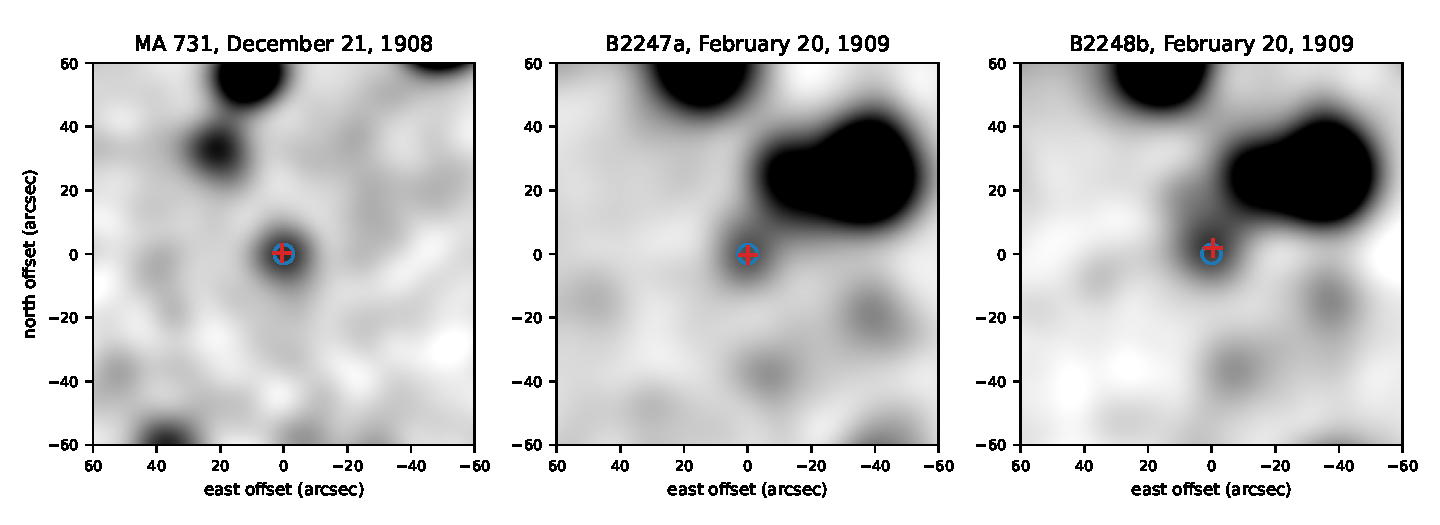
\includegraphics[width=\textwidth]{../data/stamps.pdf}
\caption{Processed close-ups of the candidate locations on MA~731 (left), B2247a and B2248b, $2'$ square, north up and east left. Each shows the scan after filtering for star-shaped signals, in units of S/N from $-2$ (white) to 8 (black), so darker gray means stronger signal. The blue circle (radius $3''$) is centered on Pluto's predicted position and the red cross marks Method B's measured image center. Scan data: Harvard College Observatory, DASCH; Landessternwarte Heidelberg-Königstuhl, HDAP.}
\label{fig:stamps}
\end{figure}

\paragraph{Motion between the epochs.}
Between the midpoints, 61 days apart, Pluto's prediction moves $3223''$ west and $428''$ north. This follows from the two position matches and is not a separate test, but it excludes a single fixed object: the December position lies off both February scans, and the February position off MA~731.

\section{Tests against other explanations}
\label{sec:tests}

Appendix~\ref{app:tests} gives the tests against fixed sources, plate flaws and known small bodies: catalogs, 67 other sensitive plates of the two positions, the image's shape, and known asteroids at nominal predicted positions.

\paragraph{Chance.}
We moved Pluto's three predicted positions together by one random offset and replayed Method B's measurement there: the brightest filtered pixel within 8 pixels, its fitted center, the S/N there, the center's distance from the moved prediction and a check for Gaia stars within $3''$. Of 300,000 offsets within $\pm1500''$, 230,352 lie more than $60''$ from the real one and inside all three cut-outs. The thresholds are the same replay's values at the real predictions: S/N 6.25, 4.84 and 5.84, and distances $0.65''$, $0.31''$ and $1.90''$.

A match on all three plates at least as close and as strong as observed occurred in 0 of 230,352 trials (95\% upper bound $1.3\times10^{-5}$). Restricting the offsets to those whose count of Gaia stars ($G<19.5$) within $60''$ is within 20\% of Pluto's on every plate leaves 0 of 39,786 (bound $7.5\times10^{-5}$). On single plates the same test is passed at rates of $1.3\times10^{-4}$ (29 trials) on MA~731, $2.6\times10^{-5}$ (6) on B2247a and $9.7\times10^{-4}$ (223) on B2248b.

The search's own acceptance rule is much looser: any S/N of at least 4 at the fitted center, wherever in the 8-pixel window it falls. Under that rule, 8,581 trials match all three plates, and in 3,360 of them (1.5\%) the center has no Gaia star within $3''$ on any plate. An earlier version of this test, which counted local maxima in a list of peaks rather than replaying the measurement, reported none of the latter; the exact replay corrects it. Most of these matches arise near bright stars just outside the window: the brightest filtered pixel lies on the star's outer profile, and the fitted center moves toward the star, a median $11''$ to $12''$ from the moved prediction, yet stays more than $3''$ from it. Requiring the center to lie within $3''$ of the moved prediction leaves 0 trials, but we chose that cut after seeing these counts.

These rates are per trial, conditional on the three plates and times reported here, their observed thresholds and these definitions; they are not probabilities that the identification is wrong. They leave out the other plates and times examined (MA~733 and the archived MA times) and how these three were selected, and they do not model plate defects. Each scan holds many uncataloged peaks with S/N within 1 of the image's (31 on MA~731 more than $2'$ from the prediction); a sheet in the repository shows each image among 11 of them in shuffled order, keyed separately. The identification rests on the position and date of the images, not on their appearance.

\section{The census of earlier plates}
\label{sec:census}

We searched DASCH DR7, the Heidelberg archive and APPLAUSE DR4 \cite{Enke2024,APPLAUSEDR4} for plates of Pluto's predicted position from 1880 to June 1909 (Appendix~\ref{app:census} gives the query geometry). The depth test differs by archive: for DASCH, its catalog limiting magnitude against Pluto's predicted $B$; for Heidelberg, which publishes no limit, the recovery of faint comparison stars or of inserted artificial images.

From December 1908 to June 1909, of 149 DASCH exposures with Pluto inside the plate, only MA~731 is deep enough by its DASCH limit, and the Heidelberg archive returns only B2247a and B2248b, which pass by injection. Among the earlier plates we could assess, none is deep enough: 525 DASCH exposures with a limit, all short of Pluto's $B$, and ten Heidelberg plates that did not reliably recover faint comparison stars. Others remain unassessed (Appendix~\ref{app:census}): 1,221 earlier DASCH exposures without a limit, 70 deep Harvard plates without a plate solution (a usable map from scan pixels to sky coordinates), 11 exposures where Pluto may lie beyond the plate edge, the Heidelberg plate B342a, and I~31266 of 1903, whose limit is 0.76 mag brighter than Pluto's $B$ and which we did not measure. Plates of other collections, such as the Yerkes plates, and plates never scanned are not covered.

\section{Limits}
\label{sec:limits}

\paragraph{The December date rests on MA~731 alone,} an image of S/N 6.3 in Method B; MA~733, less deep, neither supports nor contradicts it (Appendix~\ref{app:tests}). The scans cannot exclude a brief brightening of a source usually too faint for the modern catalogs searched, an asteroid unknown today, or a chance cluster of photographic grains, which the glass itself might distinguish. Examining the original plate is therefore the key next check.

\paragraph{The February images,} of S/N 4.8 and 5.8, come from two plates exposed together, which excludes a flaw confined to one plate but not an unknown transient or asteroid that night.

\paragraph{Known bodies and calibration.} The known-asteroid tests use nominal orbits, unreliable in 1908 for many near-Earth objects. Both methods calibrate on stars of the same plate, since 1908 emulsions are undocumented. Unscanned plates of February 1909 could add a check.

\section{Verification and reproducibility}
The released check, \texttt{checks/rerun.py}, reproduces from public data the trail clocks, Method B's measurements of the three plates and the 1914 and 1923 control plates, the faint-star comparison, the random-offset tests and the Gaia and SkyBoT checks. It compares 44 numbers with recorded ranges and fails if any falls outside; with downloads it takes about ten minutes. \texttt{checks/figure.py} draws the figure and the blinded sheet, and \texttt{checks/census.py} rebuilds the census. Appendix~\ref{app:checks} lists the 44 checked values with their tolerances, and the results that are recorded, not rerun, with their inputs.

\section*{Acknowledgments}
This work made use of data provided by Digital Access to a Sky Century @ Harvard (DASCH), which has been partially supported by NSF grants AST-0407380, AST-0909073 and AST-1313370; work on DASCH Data Release 7 received support from the Smithsonian American Women's History Initiative Pool. This work made use of the HDAP, which was produced at Landessternwarte Heidelberg-Königstuhl under grant No.~00.071.2005 of the Klaus-Tschira-Foundation. This work has made use of data from APPLAUSE Data Release 4. Funding for APPLAUSE has been provided by DFG (German Research Foundation, Grant), Leibniz Institute for Astrophysics Potsdam (AIP), Dr.~Remeis Sternwarte Bamberg (University Nuernberg/Erlangen), the Hamburger Sternwarte (University of Hamburg) and Tartu Observatory. Plate material also has been made available from Thüringer Landessternwarte Tautenburg, and from the archives of the Vatican Observatory. Other services, catalogs and software used are cited in the text.

\begin{thebibliography}{99}
\bibitem{Berthier2006} J.~Berthier, F.~Vachier, W.~Thuillot, P.~Fernique, F.~Ochsenbein, F.~Genova, V.~Lainey and J.-E.~Arlot, SkyBoT, a new VO service to identify Solar System objects, in \emph{Astronomical Data Analysis Software and Systems XV}, ASP Conf.\ Ser.\ 351 (2006), 367.
\bibitem{Bower1931} E.~C.~Bower, On the orbit and mass of Pluto with an ephemeris for 1931--1932, \emph{Lick Observatory Bulletin} 15 (1931), 171--178.
\bibitem{Brozovic2024} M.~Brozović and R.~A.~Jacobson, Post-New Horizons orbits and masses for the satellites of Pluto, \emph{Astron.\ J.} 167 (2024), 256, \href{https://doi.org/10.3847/1538-3881/ad39f0}{doi:10.3847/1538-3881/ad39f0}.
\bibitem{Buchwald2000} G.~Buchwald, M.~DiMario and W.~Wild, Pluto is discovered back in time, in \emph{Amateur--Professional Partnerships in Astronomy}, ASP Conf.\ Ser.\ 220 (2000), 355--356.
\bibitem{Buie1997} M.~W.~Buie, D.~J.~Tholen and L.~H.~Wasserman, Separate lightcurves of Pluto and Charon, \emph{Icarus} 125 (1997), 233--244, \href{https://doi.org/10.1006/icar.1996.5624}{doi:10.1006/icar.1996.5624}.
\bibitem{Buie2006} M.~W.~Buie, W.~M.~Grundy, E.~F.~Young, L.~A.~Young and S.~A.~Stern, Orbits and photometry of Pluto's satellites: Charon, S/2005 P1, and S/2005 P2, \emph{Astron.\ J.} 132 (2006), 290--298, Table~4; arXiv:astro-ph/0512491.
\bibitem{Chambers2016} K.~C.~Chambers et al., The Pan-STARRS1 surveys, arXiv:1612.05560 (2016).
\bibitem{DASCHguide} DASCH, Legacy data guide, ``Exposure start and stop times'', \url{https://dasch.cfa.harvard.edu/data-guide/} (accessed November 19, 2026).
\bibitem{DiMario2025} M.~DiMario, Before Pluto was Pluto: an accidental capture, talk at a society membership meeting, September 13, 2025, \url{https://www.mmastrosociety.org/event-details/membership-meeting-before-pluto-was-pluto-an-accidental-capture}.
\bibitem{Enke2024} H.~Enke, T.~Tuvikene, D.~Groote, H.~Edelmann and U.~Heber, Archives of Photographic PLates for Astronomical USE (APPLAUSE), \emph{Astron.\ Astrophys.} 687 (2024), A165, \href{https://doi.org/10.1051/0004-6361/202348793}{doi:10.1051/0004-6361/202348793}.
\bibitem{APPLAUSEDR4} APPLAUSE Data Release 4, Leibniz Institute for Astrophysics Potsdam, \href{https://doi.org/10.17876/plate/dr.4}{doi:10.17876/plate/dr.4}.
\bibitem{Flewelling2020} H.~A.~Flewelling et al., The Pan-STARRS1 database and data products, \emph{Astrophys.\ J.\ Suppl.} 251 (2020), 7.
\bibitem{Gaia2023} Gaia Collaboration, A.~Vallenari et al., Gaia Data Release 3: Summary of the content and survey properties, \emph{Astron.\ Astrophys.} 674 (2023), A1.
\bibitem{Giorgini1996} J.~D.~Giorgini et al., JPL's on-line Solar System data service, \emph{Bull.\ Am.\ Astron.\ Soc.} 28 (1996), 1158.
\bibitem{Grindlay2012} J.~Grindlay, S.~Tang, E.~Los and M.~Servillat, Opening the 100-year window for time-domain astronomy, in \emph{New Horizons in Time-Domain Astronomy}, Proc.\ IAU Symp.\ 285 (2012), 29--34, \href{https://doi.org/10.1017/S1743921312000166}{doi:10.1017/S1743921312000166}.
\bibitem{HDAP} H.~Mandel, K.~Birkle, M.~Demleitner and Landessternwarte Heidelberg, HDAP: Heidelberg Digitized Astronomical Plates, GAVO Data Center, \href{https://doi.org/10.21938/haTEMZmoaCTEK6XZvGU.fQ}{doi:10.21938/haTEMZmoaCTEK6XZvGU.fQ}.
\bibitem{Henden2016} A.~A.~Henden, S.~Templeton, D.~Terrell, T.~C.~Smith, S.~Levine and D.~Welch, VizieR Online Data Catalog: AAVSO Photometric All Sky Survey (APASS) DR9, II/336 (2016).
\bibitem{Holman2023} M.~J.~Holman, A.~Akmal, D.~Farnocchia, H.~Rein, M.~J.~Payne, R.~Weryk, D.~Tamayo and D.~M.~Hernandez, ASSIST: an ephemeris-quality test-particle integrator, \emph{Planet.\ Sci.\ J.} 4 (2023), 69, \href{https://doi.org/10.3847/PSJ/acc9a9}{doi:10.3847/PSJ/acc9a9}.
\bibitem{HorizonsManual} JPL Solar System Dynamics, Horizons System manual, \url{https://ssd.jpl.nasa.gov/horizons/manual.html} (accessed November 19, 2026).
\bibitem{Johnstone1932} D.~Johnstone, Remeasurement of an early Harvard photograph of Pluto, \emph{Harvard College Observatory Bulletin} 887 (1932), 13.
\bibitem{Laycock2010} S.~Laycock, S.~Tang, J.~Grindlay, E.~Los, R.~Simcoe and D.~Mink, Digital Access to a Sky Century at Harvard: initial photometry and astrometry, \emph{Astron.\ J.} 140 (2010), 1062--1077.
\bibitem{Monet2003} D.~G.~Monet et al., The USNO-B catalog, \emph{Astron.\ J.} 125 (2003), 984--993; VizieR I/284.
\bibitem{Montegriffo2023} Gaia Collaboration, P.~Montegriffo et al., \emph{Gaia Data Release 3: The Galaxy in your preferred colours. Synthetic photometry from Gaia low-resolution spectra}, Astron.\ Astrophys.\ 674 (2023), A33, \href{https://doi.org/10.1051/0004-6361/202243709}{doi:10.1051/0004-6361/202243709}; table \texttt{gaiadr3.synthetic\_photometry\_gspc}.
\bibitem{MPC} Minor Planet Center, (134340) Pluto: observations and orbit, \url{https://minorplanetcenter.net/db_search/show_object?object_id=134340} (accessed November 19, 2026).
\bibitem{Murtagh2026} J.~Murtagh, C.~O.~Chandler, M.~Jurić et al., A century-long archival search and analysis of the Rubin Observatory-discovered dwarf planet candidate 2026~ED$_{138}$, arXiv:2611.02371, posted November 2, 2026.
\bibitem{Nature1931} Orbit and mass of Pluto, \emph{Nature} 128 (1931), 1047--1048.
\bibitem{Park2021} R.~S.~Park, W.~M.~Folkner, J.~G.~Williams and D.~H.~Boggs, The JPL planetary and lunar ephemerides DE440 and DE441, \emph{Astron.\ J.} 161 (2021), 105, \href{https://doi.org/10.3847/1538-3881/abd414}{doi:10.3847/1538-3881/abd414}.
\bibitem{Reichhardt2015} T.~Reichhardt, Are these 1909 photos the oldest pictures of Pluto? Maybe., \emph{Air \& Space Magazine}, July 15, 2015, \url{https://www.smithsonianmag.com/air-space-magazine/are-these-1909-photos-oldest-known-pictures-pluto-180955930/}.
\bibitem{Rein2012} H.~Rein and S.-F.~Liu, REBOUND: an open-source multi-purpose N-body code for collisional dynamics, \emph{Astron.\ Astrophys.} 537 (2012), A128; arXiv:1110.4876.
\bibitem{Rein2015} H.~Rein and D.~Tamayo, WHFast: a fast and unbiased implementation of a symplectic Wisdom--Holman integrator for long-term gravitational simulations, \emph{Mon.\ Not.\ R.\ Astron.\ Soc.} 452 (2015), 376--388, \href{https://doi.org/10.1093/mnras/stv1257}{doi:10.1093/mnras/stv1257}.
\bibitem{SBDB} JPL Solar System Dynamics, Small-Body Database and its query and identification services, \url{https://ssd.jpl.nasa.gov/tools/sbdb_query.html} (accessed November 19, 2026).
\bibitem{Schaefer2008} B.~E.~Schaefer, M.~W.~Buie and L.~T.~Smith, Pluto's light curve in 1933--1934, \emph{Icarus} 197 (2008), 590; arXiv:0805.2097v1 (the version quoted here).
\bibitem{Shapley1932} H.~Shapley, An early Harvard photograph of Pluto, \emph{Harvard College Observatory Bulletin} 886 (1932), 4.
\bibitem{Simcoe2006} R.~J.~Simcoe, J.~E.~Grindlay, E.~J.~Los, A.~Doane, S.~G.~Laycock, D.~J.~Mink, G.~Champine and A.~Sliski, An ultrahigh-speed digitizer for the Harvard College Observatory astronomical plates, \emph{Proc.\ SPIE} 6312 (2006), 631217.
\bibitem{Skrutskie2006} M.~F.~Skrutskie et al., The Two Micron All Sky Survey (2MASS), \emph{Astron.\ J.} 131 (2006), 1163--1183; VizieR II/246.
\bibitem{Tombaugh1946} C.~W.~Tombaugh, The search for the ninth planet, Pluto, \emph{Astron.\ Soc.\ Pacific Leaflets} 5 (1946), 73.
\bibitem{Watson2006} C.~L.~Watson, A.~A.~Henden and A.~Price, The International Variable Star Index (VSX), \emph{Society for Astronomical Sciences Annual Symposium} 25 (2006), 47; VizieR B/vsx.
\bibitem{Wild1998} W.~J.~Wild, G.~Buchwald, M.~J.~DiMario and E.~M.~Standish, Serendipitous discovery of the oldest known photographic plates with images of Pluto, \emph{AAS/Division for Planetary Sciences Meeting Abstracts} 30 (1998), 55.14.
\bibitem{Williams2025} P.~K.~G.~Williams, DASCH: bringing 100+ years of photographic data into the 21st century and beyond, arXiv:2501.12977 (2025).
\bibitem{Zacharias2013} N.~Zacharias, C.~T.~Finch, T.~M.~Girard, A.~Henden, J.~L.~Bartlett, D.~G.~Monet and M.~I.~Zacharias, The fourth US Naval Observatory CCD Astrograph Catalog (UCAC4), \emph{Astron.\ J.} 145 (2013), 44; data \href{https://doi.org/10.26131/IRSA17}{doi:10.26131/IRSA17}; VizieR I/322A.
\end{thebibliography}
\begin{appendices}
\section{Tests against fixed sources, flaws and known bodies}
\label{app:tests}

\paragraph{Positions.} The predictions are Horizons topocentric astrometric positions of target 999, for Taunton ($71.0903^\circ$\,W, $41.8997^\circ$\,N, the plate record's coordinates) and for the Königstuhl (observatory code 024), with the historical clock times taken as UT1. The predictions at each method's adopted midpoint and the measured centers, in ICRF degrees, are:

\begin{center}
\footnotesize
\begin{tabular}{@{}llll@{}}
\toprule
 & MA 731 & B2247a & B2248b \\
\midrule
Method A prediction & 85.893539, $+$16.016552 & 84.961553, $+$16.133501 & 84.961599, $+$16.133479 \\
\quad at (UT) & 00:58:29 & 20:17:45 & 20:07:21 \\
Method A center & 85.893481, $+$16.016531 & 84.961402, $+$16.133058 & 84.961295, $+$16.133450 \\
\midrule
Method B prediction & 85.893540, $+$16.016552 & 84.961542, $+$16.133507 & 84.961541, $+$16.133507 \\
\quad at (UT) & 00:58:23 & 20:20:11 & 20:20:23 \\
Method B center & 85.893708, $+$16.016635 & 84.961541, $+$16.133421 & 84.961443, $+$16.134026 \\
\bottomrule
\end{tabular}
\end{center}
Method A's Heidelberg centers are reconstructed from its recorded offsets. Typical position errors are the median misses of comparably faint stars in Table~\ref{tab:measure}. Carrying the December image by Pluto's predicted motion, each method's offset from its own February predictions repeats to $0.84''$ and $1.82''$ (Method B) and $1.56''$ and $0.85''$ (Method A) on B2247a and B2248b.

\paragraph{Fixed sources.}
At the MA~731 image the nearest Gaia DR3 source of any magnitude is $11.4''$ away ($G=18.86$). 2MASS \cite{Skrutskie2006} and USNO-B1.0 \cite{Monet2003} list the same star, $11.3''$ and $11.2''$ away, and nothing closer within $15''$; UCAC4 \cite{Zacharias2013} lists nothing within $15''$, and VSX \cite{Watson2006} nothing within $60''$. At the February position the nearest Gaia source is $17.1''$ away ($G=19.84$), and none of these four catalogs lists anything within the same radii. In Pan-STARRS DR2 \cite{Chambers2016,Flewelling2020} the nearest stack object is $8.7''$ from the December image ($r=22.1$) and $14.3''$ from the February position. Our first query of the mean catalog was restricted to objects detected at least twice, in a $0.006^\circ$ ($21.6''$) cone around Method A's December center; it found nothing closer than $8.1''$ ($r=21.2$, nine detections). Without that restriction, the mean catalog lists within $15''$ only objects detected once closer than this: at the December image a single $z$-band detection $0.9''$ away, at an epoch when SkyBoT lists no known asteroid there, and at the February position four such entries, the nearest $3.4''$ away, so none would pass the two-detection filter. We quote no completeness for these catalogs at these positions. These catalog queries are recorded, not rerun.

Other plates were measured at the same sky positions with Method B. Of 87 DASCH plates of the December position, 24 others (1909--1949) would show a fixed $B=16.2$ source at S/N $\ge4$, and their S/N there runs from $-1.7$ to $+0.8$. Of 89 DASCH plates of the February position, 43 sensitive plates (1899--1953) give $-2.1$ to $+2.1$. The Heidelberg Bruce plate B4816a (December 29, 1923, 3 hours), on which Method B recovers all injected $B=16.4$ images at S/N $\ge3$, gives S/N $-0.70$ at the February position. The DASCH series are recorded, not rerun; the B4816a test is rerun.

\paragraph{MA~733 (recorded, not rerun).} Taken the next night and less deep, MA~733 shows only a 2.6--3.0$\sigma$ excess 3--4$''$ from its own prediction, mostly across Pluto's track, and no signal at the December image's position. The duplicate MB plates of both nights noted on the envelopes were never scanned and would be too shallow.

\paragraph{Plate flaws.}
On MA~731 the image's width, ellipticity and concentration lie at the 40th, 54th and 17th percentiles of 48 nearby stars of the same S/N, and its elongation follows the plate's own image shape; emulsion flaws are typically sharper. Bright stars on MA~731 show no displaced secondary image, which argues against a second, shifted exposure of the field. The two Heidelberg plates exclude a flaw confined to one plate. Still possible are a star-like grain cluster or flaw on MA~731, separate defects that happen to coincide on the two Heidelberg plates, and an artifact of scanning common to both.

\paragraph{Known small bodies.}
For December, IMCCE SkyBoT \cite{Berthier2006} lists no object other than Pluto within $1'$ of the image at the opening, middle and close of the exposure. JPL's identification service found no comet, Centaur, trans-Neptunian or other small-class body there, but could not search the near-Earth, main-belt or Trojan classes for 1908. For those we integrated back to 1908 the nominal orbits of a filtered selection from the JPL Small-Body Database \cite{SBDB}, chosen by absolute magnitude $H$ as able to reach $V\le18$ there: near-Earth objects and Mars-crossers with $H>17.3$, and asteroids of all classes with $H\le17.3$. Bodies outside that selection were not integrated. Asteroids other than near-Earth objects were integrated with REBOUND 4.6.0 \cite{Rein2012} and WHFast \cite{Rein2015}, and near-Earth objects with ASSIST 1.2.3 \cite{Holman2023}, using DE440 \cite{Park2021} and JPL's asteroid perturber file \texttt{sb441-n16}. The nominal positions put nothing besides Pluto within $6.3'$. In random samples checked against Horizons, main-belt positions agreed to a median of $2.4''$, but 15 of 63 near-Earth objects and 1 of 20 Mars-crossers differed by more than $1^\circ$, so the integration does not test those classes reliably, and we make no claim for them. Followed with Horizons, the 32 other bodies whose nominal positions fall within $1^\circ$ would have trailed $38''$--$60''$ during the exposure, while the image is star-like. For February, SkyBoT lists no object other than Pluto within $10'$ of the position from Heidelberg; no integration was made for that date. Neither test covers asteroids unknown today. The integration is recorded, not rerun.

\section{The census in detail}
\label{app:census}

Pluto's geocentric position and $V$ came from Horizons daily, with $B=V+0.87$, the redder assumed color; its $B$ over these years runs from 16.4 to 16.8. With the adopted combined 1933--34 color, 0.78, Pluto is 0.09 mag brighter and every margin below rises by 0.09 mag: MA~733 ($-0.09$) and I~31266 ($-0.67$) remain short, no other DASCH exposure passes, and the result is unchanged (\texttt{census.json} reports both).

\paragraph{DASCH.} Pluto's track was sampled every 30 days, and a sample was skipped when Pluto was within $30^\circ$ of the Sun on the sample date. At each kept sample the DASCH exposure query asked for exposures with midpoints within 15 days that cover the sample point, whatever Pluto's elongation on their own dates. Exposures whose dates fall only in the windows of skipped samples were not queried. Each returned exposure was then placed against Pluto's position at its own date. It counts as inside when DASCH's edge distance at the sample point exceeds Pluto's distance from that point, as edge (unresolved) when the edge distance is equal or smaller, and as unknown when DASCH gives no edge distance. A plate that covers Pluto on its date but not the sample point is missed. A row is one plate solution's exposure; an exposure returned by several samples is kept once with its best label (inside, then edge, then unknown). Merging the rows of different plate solutions of the same exposure in the same way leaves every count below unchanged. A plate's depth margin is DASCH's limiting magnitude (from APASS, else ATLAS) minus Pluto's $B$, both unrounded; the code tests for a missing limit before the comparison, and a margin of zero or more passes. No margin lies within 0.17 mag of zero, so no verdict depends on rounding. \texttt{data/census-exposures.csv}, written by \texttt{checks/census.py} (SHA-256 \texttt{1d2dda36fd391404}\ldots), lists all 1,906 DASCH exposures counted here, one row per exposure, with plate, date, series, plate solution, coverage, limit, Pluto's $B$, margin and verdict.

From December 1908 to June 1909, 149 exposures cover Pluto by this test, none is unresolved, and 56 have a limit. Only MA~731 passes (margin $+0.47$); MA~733 is $0.18$ mag short, and the rest a magnitude or more.

Before December 1908, 1,746 exposures from 1886 on cover Pluto by this test; for 11 more, the edge distance is smaller than Pluto's distance from the sample point, so whether they cover Pluto is unresolved, and none lacks an edge distance. Of the 1,746, 525 have a limit and none passes. The deepest, I~31266 (December 14, 1903, 63 minutes), has a limit 0.76 mag brighter than Pluto's $B$; on the scan it expects S/N 3.6 where MA~731 expects 4.1, so a non-detection there would say little, and we did not measure it. Eight plates of the deep series without a DASCH limit fail a depth screen on their scans. Seventy plates of the deep B, C and I series of 30 minutes or more have no plate solution, that is, no usable map from scan pixels to sky coordinates, and were not screened.

\paragraph{Heidelberg.} The archive's plate table was searched for plates centered at RA $30^\circ$--$110^\circ$ and Dec $-10^\circ$ to $+35^\circ$ before July 1909, and Pluto placed on each with the archive's plate solution. Besides B2247a and B2248b, which recover inserted artificial images about 0.5 mag fainter than Pluto, Pluto falls on ten plates from Wolf's double astrograph (1896 and 1901) and the Bruce plate B342a (1901). The double-astrograph plates did not reliably recover faint comparison stars. On B342a Pluto lies 75 pixels from the scan edge, and the plate could not be registered there.

\paragraph{APPLAUSE.} The DR4 exposure table lists 34 exposures before mid-1909 with a recorded time and pointing, all from Potsdam (1893--1902). The nearest nominal pointing is $22.9^\circ$ from Pluto at its date.

\section{Exposure times in detail}
\label{app:clock}

The (179) Klytaemnestra estimate models the signal along the asteroid's JPL track, one point per minute, as a band with blurred start and stop edges, in a square of $\pm0.2^\circ$ around the track. It gives an opening at $00{:}21.9\pm1.2$, a closing at $01{:}34.8\pm0.5$ and a midpoint at $00{:}58.4\pm0.7$ UT. These $1\sigma$ errors come from the fit, inflated for the correlation of neighboring minutes, and are conditional on the model. Fits to the weaker trails of (1436) Salonta and (2891) McGetchin give 01:01.5 and 01:04.2 UT, and combined measurements along the tracks of eight fainter asteroids peak at 01:02.5 UT. Of those eight, four of the seven testable on MA~731 show excess signal in the estimated window ($p\le0.004$) and none of the five testable in the archived window; on MA~733 four of eight do. (An earlier version reported 9 of 15 pairs pooled over both plates; the recorded tests give 8.) A 60-minute exposure that began at the fitted opening or ended at the fitted closing would shift the midpoint by 6.5 minutes either way.

Why the archived time differs is not known. If the logbook's start, kept in sidereal time (a clock set by the stars), was read as local mean time (a clock set by the Sun), the archived midpoint is reproduced to 2 minutes; this is untested against the logbook, and the same reading does not reproduce MA~733.

At Heidelberg, Method B's fits to the trail of (417) Suevia, $2.3^\circ$ from Pluto, place the midpoints $0\pm3.5$ and $-7\pm5$ minutes from the archived times; other trails gave Method B no clean fit. Method A fitted the trails of (168) Sibylla and (417) Suevia on both plates and (179) Klytaemnestra on B2248b, and adopts the median on each plate.

\section{Earlier prediscovery reports}
\label{app:history}

Lowell's search for a trans-Neptunian planet had recorded Pluto on Flagstaff plates in 1915 without recognizing it \cite{Nature1931}. Bower mentions ``the probable 1903 observation by Franklin-Adams announced last January'' \cite{Bower1931}; a contemporary summary adds that P.~J. Melotte, who detected this image, ``now considers that it is too ill-defined and doubtful to use'' \cite{Nature1931}. On the Harvard plate MC~6858 of November 1914, Arville D. Walker found an image near the plate's limit after Bower communicated an ephemeris; Constance D. Boyd measured it, and Bower derived its position \cite{Shapley1932}; it was later remeasured \cite{Johnstone1932}. Schaefer, Buie and Smith examined that plate and saw only ``a `grain enhancement' similar to many in the area'', and recommended removing it from the list \cite[Section~6]{Schaefer2008}. Of the Yerkes images of 1909, M.~DiMario gave a public talk, ``Before Pluto was Pluto: An Accidental Capture'', on September 13, 2025 \cite{DiMario2025}; we found no publication of measured positions.

\section{What the released check covers}
\label{app:checks}

\texttt{checks/rerun.py} compares the 44 values of Table~\ref{tab:checks}, recorded on November 19, 2026, with the tolerances shown, and fails if any falls outside; the list is \texttt{data/expected.json}. Other values it writes are not checked. The figure and blinded sheet are drawn by \texttt{python checks/figure.py WORK OUT.svg} and \texttt{python checks/figure.py WORK OUT.pdf -{}-blind KEY.json} from inputs that \texttt{rerun.py} saves.

\begin{table}[p]
\centering
\scriptsize
\begin{tabular}{@{}rp{0.70\textwidth}l@{}}
\toprule
 & Value & Tolerance \\
\midrule
1 & MA 731 clock correction from (179) Klytaemnestra, minutes (recorded -348.2) & $-$353 to $-$343 \\
2 & MA 731 fitted exposure length, minutes (recorded 72.9; storage envelope 60) & 60 to 85 \\
3 & MA 731 S/N at the free centroid (recorded 6.25) & $\ge$ 5.5 \\
4 & MA 731 centroid offset from Pluto's prediction, arcsec (recorded 0.65) & $\le$ 1.2 \\
5 & MA 731 blue magnitude (recorded 16.19; predicted 16.33-16.42) & 15.8 to 16.6 \\
6 & MA 731 nearest Gaia DR3 star (G $<$ 19.5) to the image, arcsec (recorded 11.4) & $\ge$ 10 \\
7 & MA 731 S/N at the archive-time position (recorded -0.2) & $\le$ 2 \\
8 & Joint random offsets, MA 731 alone: offsets with a replayed match as close and as strong as the image (recorded 29 of 230352) & $\le$ 60 \\
9 & Same on B2247a alone (recorded 6) & $\le$ 20 \\
10 & Same on B2248b alone (recorded 223) & $\le$ 400 \\
11 & SkyBoT objects within 0.04 deg of the MA 731 image & equals Pluto \\
12 & B2247a clock from (417) Suevia minus archive midpoint, minutes (recorded 0.0) & $-$30 to 30 \\
13 & B2248b clock from (417) Suevia minus archive midpoint, minutes (recorded -6.7) & $-$30 to 30 \\
14 & B2247a S/N at the free centroid (recorded 4.84) & $\ge$ 4.3 \\
15 & B2247a centroid offset, arcsec (recorded 0.31) & $\le$ 1.2 \\
16 & B2247a blue magnitude (recorded 16.60; predicted 16.40-16.49) & 16.1 to 16.9 \\
17 & B2248b S/N at the free centroid (recorded 5.84) & $\ge$ 5.2 \\
18 & B2248b centroid offset, arcsec (recorded 1.90) & $\le$ 2.0 \\
19 & B2248b blue magnitude (recorded 16.35) & 16.0 to 16.8 \\
20 & B2247a nearest Gaia DR3 star (G $<$ 19.5), arcsec (recorded 25.6) & $\ge$ 20 \\
21 & SkyBoT objects within 0.04 deg of the February position, from Heidelberg & equals Pluto \\
22 & December image carried by Pluto's motion, miss on B2247a, arcsec (recorded 0.84) & $\le$ 2.5 \\
23 & December image carried by Pluto's motion, miss on B2248b, arcsec (recorded 1.82) & $\le$ 2.5 \\
24 & Joint random offsets: replayed matches on all three plates as close and as strong as observed (recorded 0 of 230352) & $\le$ 0 \\
25 & Joint random offsets: trials inside all three cut-outs (recorded 230352) & $\ge$ 200000 \\
26 & Joint random offsets: matches on both February plates (recorded 1) & $\le$ 5 \\
27 & Joint random offsets: matches on all three plates with no Gaia star within 3 arcsec (recorded 0) & $\le$ 0 \\
28 & 1914 positive check B3383a: S/N at the free centroid (recorded 6.80) & $\ge$ 6.0 \\
29 & 1914 positive check B3383a: offset, arcsec (recorded 1.55) & $\le$ 2.5 \\
30 & 1923 plate B4816a at the February position: S/N (recorded -0.70) & $\le$ 2 \\
31 & 1923 plate B4816a: recovery of injected B 16.4 images at S/N $\ge$ 3 (recorded 1.00) & $\ge$ 0.9 \\
32 & MA 731 clock: the trail fit reads no pixel within 1 degree of Pluto (recorded 5.38 deg) & $\ge$ 1.0 \\
33 & MA 731 clock: 1-sigma error of the fitted midpoint, minutes (recorded 0.66) & $\le$ 2.0 \\
34 & MA 731: Pluto's prediction moves this far per 1-sigma clock error, arcsec (recorded 0.03) & $\le$ 0.1 \\
35 & Heidelberg clocks read no pixel within 1 degree of Pluto (recorded 2.25 deg) & $\ge$ 1.0 \\
36 & MA 731: fraction of comparably faint catalog stars whose centroid misses by no more than the image's (recorded 0.20) & $\le$ 0.5 \\
37 & B2247a: same fraction (recorded 0.06) & $\le$ 0.5 \\
38 & B2248b: same fraction (recorded 0.73) & $\le$ 0.95 \\
39 & MA 731: robust spread of calibrated minus catalog B for comparably faint stars (recorded 0.21) & $\le$ 0.35 \\
40 & Joint random offsets with the search's loose rule (S/N $\ge$ 4 at the replayed centroid), all three plates (recorded 8581) & 6000 to 11000 \\
41 & Same, with no Gaia star within 3 arcsec of the centroid on any plate (recorded 3360) & 2000 to 5000 \\
42 & Same, centroid also within 3 arcsec of the shifted prediction, a cut chosen after seeing the data (recorded 0) & $\le$ 0 \\
43 & Joint random offsets with crowding matched to Pluto's, all three plates (recorded 0 of 39786) & $\le$ 0 \\
44 & Crowding-matched trials (recorded 39786) & $\ge$ 30000 \\
\bottomrule
\end{tabular}
\caption{The values \texttt{checks/rerun.py} checks, from \texttt{data/expected.json}.}
\label{tab:checks}
\end{table}

Recorded, not rerun by the released scripts, with their inputs (all public, read on November 19, 2026, and documented in \texttt{checks/README.md}):
\begin{itemize}
\item Method A: the DASCH scan \texttt{ma00731} and the HDAP scans of B2247a and B2248b, Gaia DR3 and its synthetic photometry, APASS DR9; separate code.
\item MA~733 and its clock: the DASCH scan \texttt{ma00733}, Method B code with its own trail fit.
\item The DASCH plates at the two fixed positions: DASCH DR7 scans and limits of the 87 and 89 plates returned at those positions, measured with Method B code.
\item The deep catalogs: VizieR tables II/246, I/322A, I/284, B/vsx and I/355, and the MAST Pan-STARRS DR2 mean and stack catalogs.
\item The known-asteroid integration: JPL Small-Body Database elements at JD 2461200.5, REBOUND 4.6.0, ASSIST 1.2.3, JPL's DE440 file \texttt{linux\_p1550p2650.440}, its asteroid perturber file \texttt{sb441-n16.bsp}, and Horizons.
\item The image-shape percentiles, the weaker trail fits of (1436) and (2891), and the combined faint-asteroid timing: the DASCH scan \texttt{ma00731} and Horizons tracks.
\end{itemize}

\end{appendices}

\end{document}
